\documentclass{standalone}
\usepackage{tikz}
\usetikzlibrary{patterns, positioning}

\begin{document}
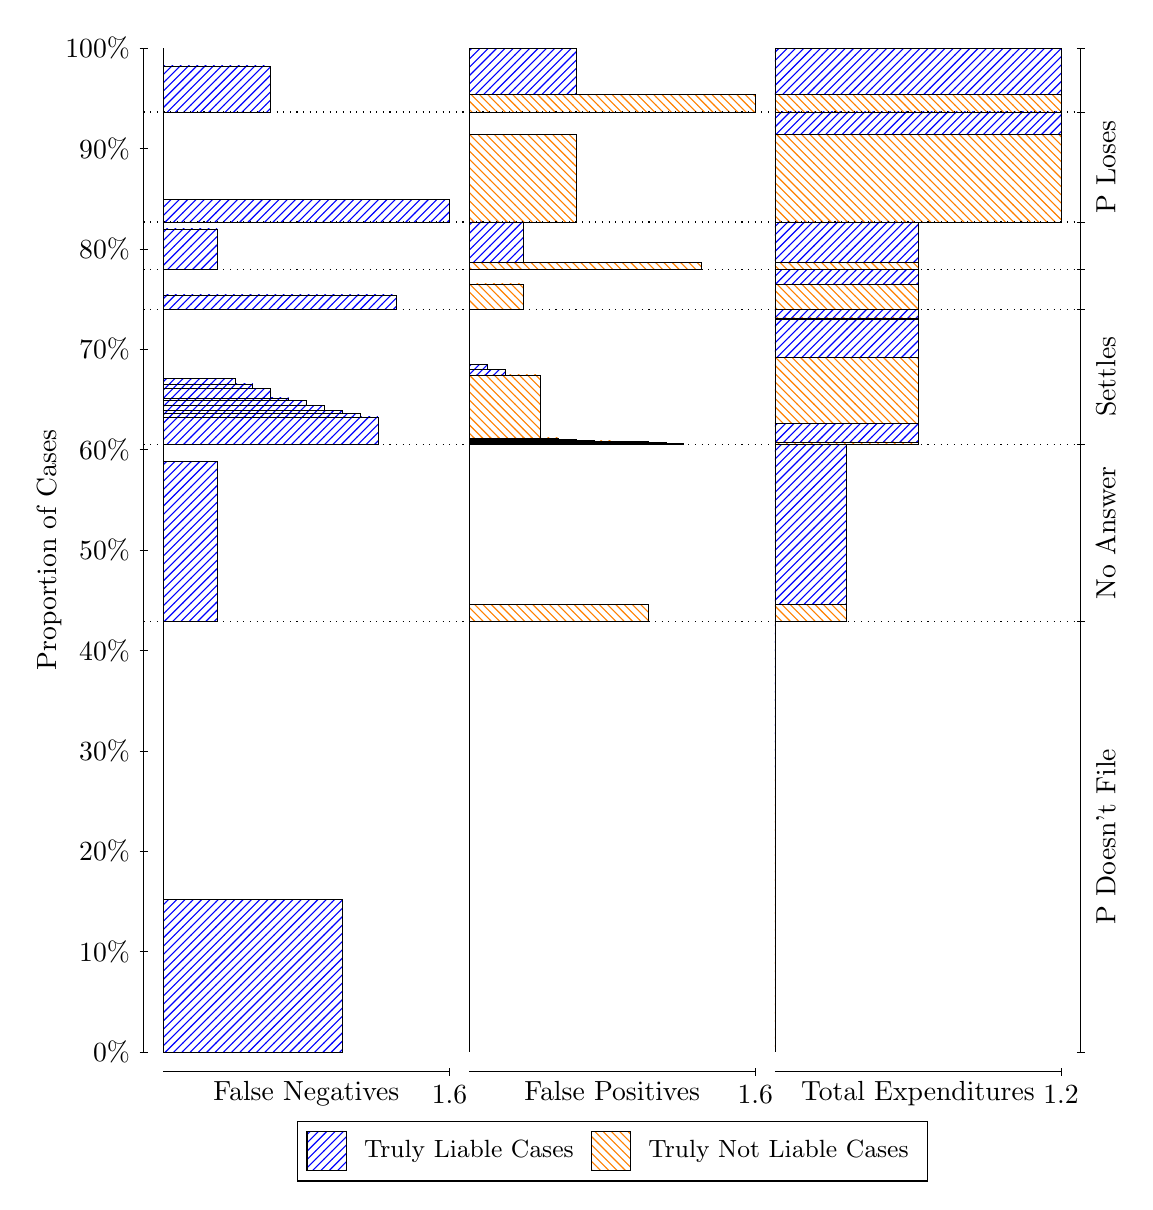
\begin{tikzpicture}
\draw[black, very thin] (1.5,1.75) -- (1.5,14.5);
\node[rotate=90, anchor=center] at (0.3, 8.125) {Proportion of Cases};
\draw[black, very thin] (1.45,1.75) -- (1.55,1.75);
\node[anchor=east] at (1.45, 1.75) {0\%};
\draw[black, very thin] (1.45,3.025) -- (1.55,3.025);
\node[anchor=east] at (1.45, 3.025) {10\%};
\draw[black, very thin] (1.45,4.3) -- (1.55,4.3);
\node[anchor=east] at (1.45, 4.3) {20\%};
\draw[black, very thin] (1.45,5.575) -- (1.55,5.575);
\node[anchor=east] at (1.45, 5.575) {30\%};
\draw[black, very thin] (1.45,6.85) -- (1.55,6.85);
\node[anchor=east] at (1.45, 6.85) {40\%};
\draw[black, very thin] (1.45,8.125) -- (1.55,8.125);
\node[anchor=east] at (1.45, 8.125) {50\%};
\draw[black, very thin] (1.45,9.4) -- (1.55,9.4);
\node[anchor=east] at (1.45, 9.4) {60\%};
\draw[black, very thin] (1.45,10.675) -- (1.55,10.675);
\node[anchor=east] at (1.45, 10.675) {70\%};
\draw[black, very thin] (1.45,11.95) -- (1.55,11.95);
\node[anchor=east] at (1.45, 11.95) {80\%};
\draw[black, very thin] (1.45,13.225) -- (1.55,13.225);
\node[anchor=east] at (1.45, 13.225) {90\%};
\draw[black, very thin] (1.45,14.5) -- (1.55,14.5);
\node[anchor=east] at (1.45, 14.5) {100\%};

\draw[black, very thin] (13.4,1.75) -- (13.4,14.5);
\draw[black, very thin] (13.35,1.75) -- (13.45,1.75);
\node[anchor=west] at (13.35, 1.75) {};
\draw[black, very thin] (13.35,7.2167) -- (13.45,7.2167);
\node[anchor=west] at (13.35, 7.2167) {};
\draw[black, very thin] (13.35,9.4704) -- (13.45,9.4704);
\node[anchor=west] at (13.35, 9.4704) {};
\draw[black, very thin] (13.35,11.184) -- (13.45,11.184);
\node[anchor=west] at (13.35, 11.184) {};
\draw[black, very thin] (13.35,11.685) -- (13.45,11.685);
\node[anchor=west] at (13.35, 11.685) {};
\draw[black, very thin] (13.35,12.291) -- (13.45,12.291);
\node[anchor=west] at (13.35, 12.291) {};
\draw[black, very thin] (13.35,13.688) -- (13.45,13.688);
\node[anchor=west] at (13.35, 13.688) {};
\draw[black, very thin] (13.35,14.5) -- (13.45,14.5);
\node[anchor=west] at (13.35, 14.5) {};

\draw[black, very thin, pattern color=blue, pattern=north east lines] (1.75,1.75) rectangle (4.0208,3.6869);
\draw[black, very thin, pattern color=orange, pattern=north west lines] (1.75,3.6869) rectangle (1.75,7.2167);
\draw[black, very thin, pattern color=blue, pattern=north east lines] (1.75,7.2167) rectangle (2.4312,9.2488);
\draw[black, very thin, pattern color=orange, pattern=north west lines] (1.75,9.2488) rectangle (1.75,9.4704);
\draw[black, very thin, pattern color=blue, pattern=north east lines] (1.75,9.4704) rectangle (4.475,9.8155);
\draw[black, very thin, pattern color=blue, pattern=north east lines] (1.75,9.8155) rectangle (4.2479,9.8586);
\draw[black, very thin, pattern color=blue, pattern=north east lines] (1.75,9.8586) rectangle (4.0208,9.8995);
\draw[black, very thin, pattern color=blue, pattern=north east lines] (1.75,9.8995) rectangle (3.7937,9.9579);
\draw[black, very thin, pattern color=blue, pattern=north east lines] (1.75,9.9579) rectangle (3.7937,9.9663);
\draw[black, very thin, pattern color=blue, pattern=north east lines] (1.75,9.9663) rectangle (3.5667,10.026);
\draw[black, very thin, pattern color=blue, pattern=north east lines] (1.75,10.026) rectangle (3.3396,10.057);
\draw[black, very thin, pattern color=blue, pattern=north east lines] (1.75,10.057) rectangle (3.1125,10.177);
\draw[black, very thin, pattern color=blue, pattern=north east lines] (1.75,10.177) rectangle (2.8854,10.234);
\draw[black, very thin, pattern color=blue, pattern=north east lines] (1.75,10.234) rectangle (2.6583,10.306);
\draw[black, very thin, pattern color=orange, pattern=north west lines] (1.75,10.306) rectangle (1.75,11.184);
\draw[black, very thin, pattern color=blue, pattern=north east lines] (1.75,11.184) rectangle (4.7021,11.366);
\draw[black, very thin, pattern color=orange, pattern=north west lines] (1.75,11.366) rectangle (1.75,11.685);
\draw[black, very thin, pattern color=blue, pattern=north east lines] (1.75,11.685) rectangle (2.4312,12.203);
\draw[black, very thin, pattern color=orange, pattern=north west lines] (1.75,12.203) rectangle (1.75,12.291);
\draw[black, very thin, pattern color=blue, pattern=north east lines] (1.75,12.291) rectangle (5.3833,12.577);
\draw[black, very thin, pattern color=orange, pattern=north west lines] (1.75,12.577) rectangle (1.75,13.688);
\draw[black, very thin, pattern color=blue, pattern=north east lines] (1.75,13.688) rectangle (3.1125,14.273);
\draw[black, very thin, pattern color=orange, pattern=north west lines] (1.75,14.273) rectangle (1.75,14.5);
\draw[black, very thin, pattern color=orange, pattern=north west lines] (5.6333,1.75) rectangle (5.6333,5.2798);
\draw[black, very thin, pattern color=blue, pattern=north east lines] (5.6333,5.2798) rectangle (5.6333,7.2167);
\draw[black, very thin, pattern color=orange, pattern=north west lines] (5.6333,7.2167) rectangle (7.9042,7.4382);
\draw[black, very thin, pattern color=blue, pattern=north east lines] (5.6333,7.4382) rectangle (5.6333,9.4704);
\draw[black, very thin, pattern color=orange, pattern=north west lines] (5.6333,9.4704) rectangle (8.3583,9.4795);
\draw[black, very thin, pattern color=orange, pattern=north west lines] (5.6333,9.4795) rectangle (8.1313,9.4868);
\draw[black, very thin, pattern color=orange, pattern=north west lines] (5.6333,9.4868) rectangle (7.9042,9.5);
\draw[black, very thin, pattern color=orange, pattern=north west lines] (5.6333,9.5) rectangle (7.6771,9.5038);
\draw[black, very thin, pattern color=orange, pattern=north west lines] (5.6333,9.5038) rectangle (7.45,9.5121);
\draw[black, very thin, pattern color=orange, pattern=north west lines] (5.6333,9.5121) rectangle (7.2229,9.5208);
\draw[black, very thin, pattern color=orange, pattern=north west lines] (5.6333,9.5208) rectangle (6.9958,9.5289);
\draw[black, very thin, pattern color=orange, pattern=north west lines] (5.6333,9.5289) rectangle (6.7687,9.5476);
\draw[black, very thin, pattern color=orange, pattern=north west lines] (5.6333,9.5476) rectangle (6.5417,10.349);
\draw[black, very thin, pattern color=blue, pattern=north east lines] (5.6333,10.349) rectangle (6.0875,10.421);
\draw[black, very thin, pattern color=blue, pattern=north east lines] (5.6333,10.421) rectangle (5.8604,10.478);
\draw[black, very thin, pattern color=blue, pattern=north east lines] (5.6333,10.478) rectangle (5.6333,11.184);
\draw[black, very thin, pattern color=orange, pattern=north west lines] (5.6333,11.184) rectangle (6.3146,11.504);
\draw[black, very thin, pattern color=blue, pattern=north east lines] (5.6333,11.504) rectangle (5.6333,11.685);
\draw[black, very thin, pattern color=orange, pattern=north west lines] (5.6333,11.685) rectangle (8.5854,11.773);
\draw[black, very thin, pattern color=blue, pattern=north east lines] (5.6333,11.773) rectangle (6.3146,12.291);
\draw[black, very thin, pattern color=orange, pattern=north west lines] (5.6333,12.291) rectangle (6.9958,13.402);
\draw[black, very thin, pattern color=blue, pattern=north east lines] (5.6333,13.402) rectangle (5.6333,13.688);
\draw[black, very thin, pattern color=orange, pattern=north west lines] (5.6333,13.688) rectangle (9.2667,13.916);
\draw[black, very thin, pattern color=blue, pattern=north east lines] (5.6333,13.916) rectangle (6.9958,14.5);
\draw[black, very thin, pattern color=orange, pattern=north west lines] (9.5167,1.75) rectangle (9.5167,5.2798);
\draw[black, very thin, pattern color=blue, pattern=north east lines] (9.5167,5.2798) rectangle (9.5167,7.2167);
\draw[black, very thin, pattern color=orange, pattern=north west lines] (9.5167,7.2167) rectangle (10.425,7.4382);
\draw[black, very thin, pattern color=blue, pattern=north east lines] (9.5167,7.4382) rectangle (10.425,9.4704);
\draw[black, very thin, pattern color=orange, pattern=north west lines] (9.5167,9.4704) rectangle (11.333,9.4992);
\draw[black, very thin, pattern color=blue, pattern=north east lines] (9.5167,9.4992) rectangle (11.333,9.7353);
\draw[black, very thin, pattern color=orange, pattern=north west lines] (9.5167,9.7353) rectangle (11.333,10.571);
\draw[black, very thin, pattern color=blue, pattern=north east lines] (9.5167,10.571) rectangle (11.333,11.058);
\draw[black, very thin, pattern color=orange, pattern=north west lines] (9.5167,11.058) rectangle (11.333,11.072);
\draw[black, very thin, pattern color=blue, pattern=north east lines] (9.5167,11.072) rectangle (11.333,11.184);
\draw[black, very thin, pattern color=orange, pattern=north west lines] (9.5167,11.184) rectangle (11.333,11.504);
\draw[black, very thin, pattern color=blue, pattern=north east lines] (9.5167,11.504) rectangle (11.333,11.685);
\draw[black, very thin, pattern color=orange, pattern=north west lines] (9.5167,11.685) rectangle (11.333,11.773);
\draw[black, very thin, pattern color=blue, pattern=north east lines] (9.5167,11.773) rectangle (11.333,12.291);
\draw[black, very thin, pattern color=orange, pattern=north west lines] (9.5167,12.291) rectangle (13.15,13.402);
\draw[black, very thin, pattern color=blue, pattern=north east lines] (9.5167,13.402) rectangle (13.15,13.688);
\draw[black, very thin, pattern color=orange, pattern=north west lines] (9.5167,13.688) rectangle (13.15,13.916);
\draw[black, very thin, pattern color=blue, pattern=north east lines] (9.5167,13.916) rectangle (13.15,14.5);
\draw[black, dotted] (1.5,7.2167) -- (13.4,7.2167);
\draw[black, dotted] (1.5,9.4704) -- (13.4,9.4704);
\draw[black, dotted] (1.5,11.184) -- (13.4,11.184);
\draw[black, dotted] (1.5,11.685) -- (13.4,11.685);
\draw[black, dotted] (1.5,12.291) -- (13.4,12.291);
\draw[black, dotted] (1.5,13.688) -- (13.4,13.688);
\draw[black, very thin] (1.75,1.5) -- (5.3833,1.5);
\node[anchor=north] at (3.5667, 1.5) {False Negatives};
\draw[black, very thin] (5.3833,1.45) -- (5.3833,1.55);
\node[anchor=north] at (5.3833, 1.45) {1.6};

\draw[black, very thin] (5.6333,1.5) -- (9.2667,1.5);
\node[anchor=north] at (7.45, 1.5) {False Positives};
\draw[black, very thin] (9.2667,1.45) -- (9.2667,1.55);
\node[anchor=north] at (9.2667, 1.45) {1.6};

\draw[black, very thin] (9.5167,1.5) -- (13.15,1.5);
\node[anchor=north] at (11.333, 1.5) {Total Expenditures};
\draw[black, very thin] (13.15,1.45) -- (13.15,1.55);
\node[anchor=north] at (13.15, 1.45) {1.2};

\node[black, centered, rotate=90] at (13.72, 4.4833) {P Doesn't File};
\node[black, centered, rotate=90] at (13.72, 8.3435) {No Answer};
\node[black, centered, rotate=90] at (13.72, 10.327) {Settles};


\node[black, centered, rotate=90] at (13.72, 12.99) {P Loses};


\draw (7.449999999999999,1.5) node[draw=none] (baseCoordinate) {};
\begin{scope}[align=center]
        \matrix[scale=0.5, draw=black, below=0.5cm of baseCoordinate, nodes={draw}, column sep=0.1cm]{
            \node[rectangle, draw, minimum width=0.5cm, minimum height=0.5cm, pattern=north east lines, pattern color=blue] {}; &
            \node[draw=none, font=\small] (B) {Truly Liable Cases}; &
            \node[rectangle, draw, minimum width=0.5cm, minimum height=0.5cm, pattern=north west lines, pattern color=orange] {}; &
            \node[draw=none, font=\small] (B) {Truly Not Liable Cases}; \\
            };
\end{scope}

\end{tikzpicture}
\end{document}